\chapter{Convolutional Neural Networks}
\label{ch5_cnn}

Convolutional Neutral Network (CNN) is a classification of multi-layered neural networks \cite{cnn_lecun_lenet5}. CNNs have excellent performance in areas such as image recognition and classification.  CNNs are at the core of state-of-the-art approaches to a variety of computer vision tasks, including image classification \cite{kriz_suts_hinton_nips2012} and object detection \cite{gir_don_dar_mal_cvpr2014}. They are widely used in the detection and identification of faces, objects and animals, apart from powering robot vision and driverless cars \cite{cnn_karn}. LeNet-5 is one such convolutional network designed for handwritten and machine-printed character and digit recognition.

\section{Introduction}
\label{sect5_1}

\subsection{Neural Networks}
\label{sect5_1_1}
An Artificial Neural Network, simply put as Neural Network, is a computational model motivated by the manner in which neural networks in the human brain and nervous system process information \cite{cnn_karn}. The field of Neural Networks was primarily inspired by the objective of modeling biological neural systems, but has since diverged and become a part of engineering and achieving great results in machine learning \cite{nn_stanford_1}. \newline\newline The fundamental building block of a neural network is the neuron, also referred to as node. The following figures shows a biological neuron and its computational model are related: \newline

\begin{figure}[h!]
\centering
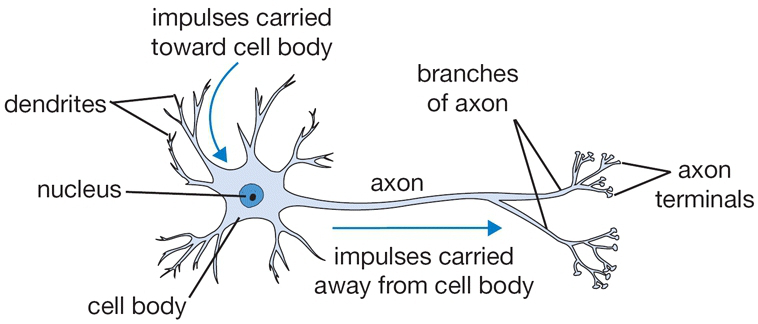
\includegraphics[width=8cm]{figures/neuron.png}
\caption{Representation of a biological neuron\cite{nn_stanford_1}}
\label{fig:cnn1}
\end{figure}

\begin{figure}[h!]
\centering
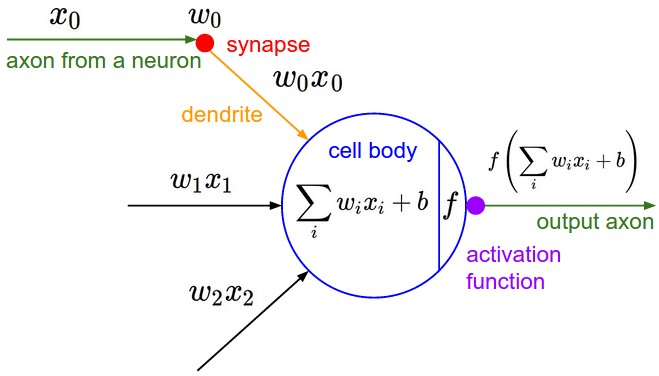
\includegraphics[width=7cm]{figures/neuron_model.jpg}
\caption{Computational model of a neuron \cite{nn_stanford_1}}
\label{fig:cnn2}
\end{figure}

In this model, a node gets inputs from other node or an external source, and calculates an output. Inputs have associated weights assigned on basis of their relevance to other input nodes. The node applies a function on the weighted sum of inputs, as shown in Figure \ref{fig:cnn3}.
\begin{figure}[h!]
\centering
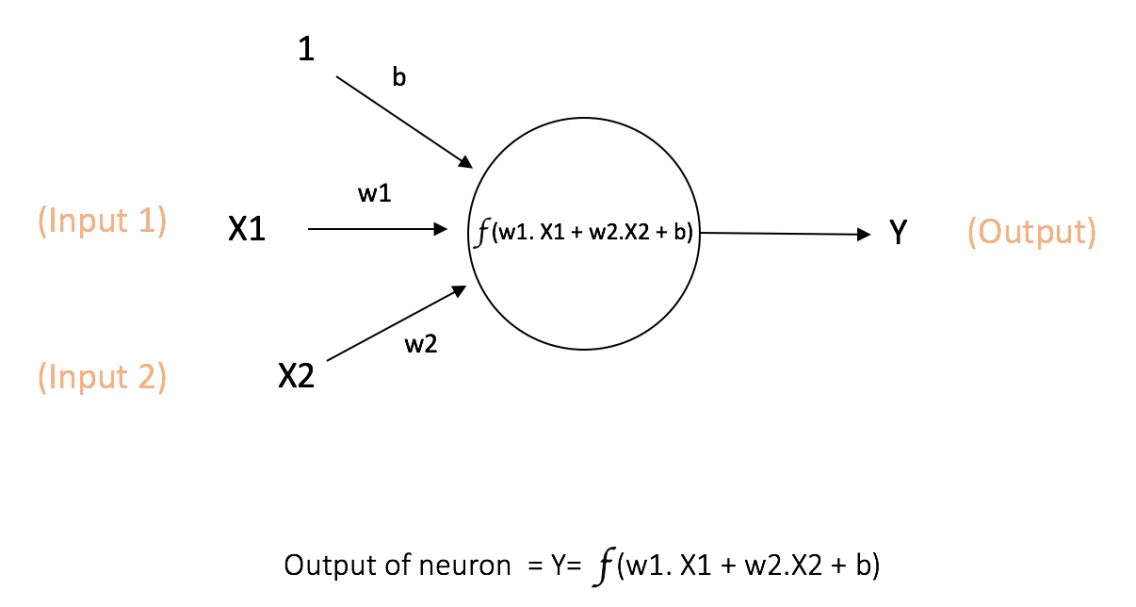
\includegraphics[width=10cm]{figures/Input_and_Output_to_a_Node.png}
\caption{Computation in a Neuron\cite{nn_karn}}
\label{fig:cnn3}
\end{figure}

The neuron receives inputs x1 and x2 with weights w1 and w2. Each neuron also has another input 1, with a weight \textbf{bias} associated with it. The bias value provides each node a trainable constant value.\newline\newline 
The function applied to the sum of weighted inputs, known as Activation Function, is a non-linear function introduced to force neurons to learn non-linear representations, as most of real world data is non-linear. Following are some common activation functions used:

\begin{itemize}
\item Sigmoid \newline
Takes a real-valued input and squeezes it in the range 0 to 1
\begin{equation}
\mathbf{\sigma(x) = 1 / (1 + exp(-x))}
\end{equation}

\item tanh \newline
Takes a real-valued input and squeezes it in the range -1 to 1
\begin{equation}
\mathbf{tanh(x) = 2 \sigma (2x)-1}
\end{equation}

\item ReLU \newline
Takes a real-valued input and thresholds it at zero (replaces negative values with zero)
f(x) = max(0, x)
\begin{equation}
\mathbf{f(x) = max(0, x)}
\end{equation}
\end{itemize}

\subsubsection{Feedforward Neural Network}
\label{sect5_1_1_1}
One of the first and simplest neural networks devised was the feedforward neural network. There are multiple neurons placed in layers, with edges connecting them. Each of these edges are tagged a weight. Figure \ref{fig:cnn4} shows an example of a feedforward neural network.\newline\newline
\begin{figure}[h!]
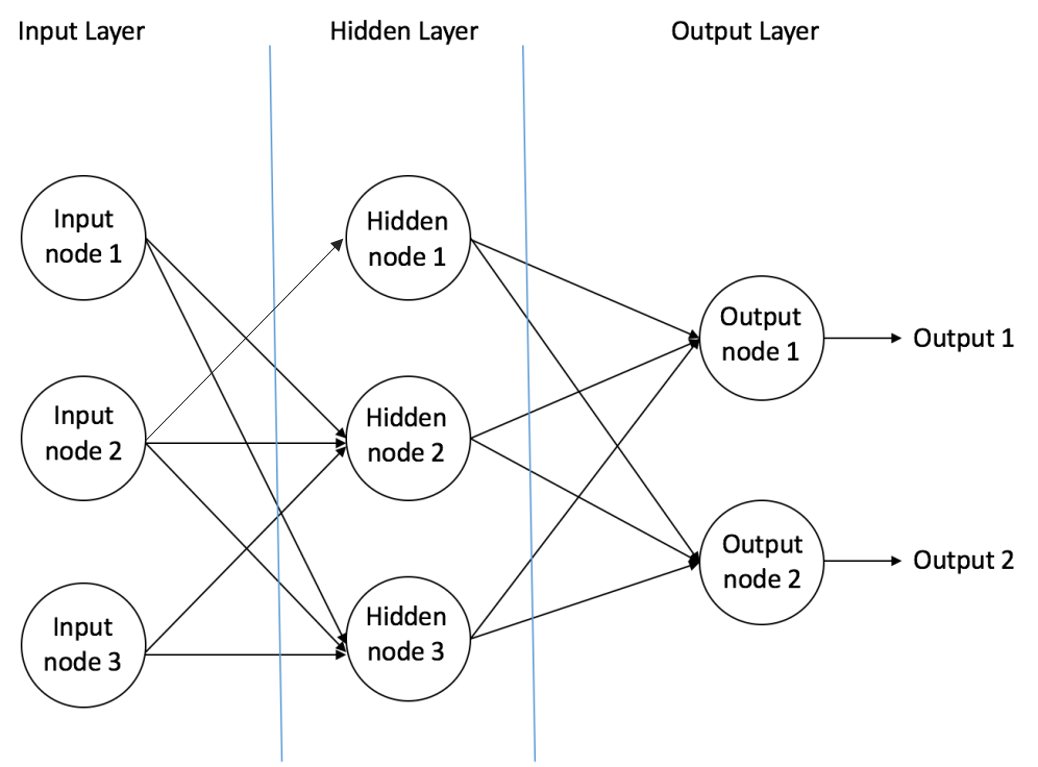
\includegraphics[width=14cm]{figures/Feedforward_Neural_Network.png}
\caption{Feedforward Neural Network \cite{nn_karn}}
\label{fig:cnn4}
\end{figure}
Information only moves in the forward direction in a feedforward neural network. Input nodes receive signals from the outside world and pass on the information forward to the hidden nodes, which perform computations and propagate information to the output nodes. The output nodes carry out some calculations and transfer the result to the outside world. There can only be one input and output layer of nodes, but multiple hidden layers of nodes in a feedforward neural network.\newline\newline 
They are of two types, \textbf{Single Layer Perceptron} and \textbf{Multi Layer Perceptron} (MLP). The former does not consist of any hidden nodes in the middle, while the the latter has at least one hidden layer. MLPs are very useful in several practical learning applications.
\subsubsection{Training}
\label{sect5_1_1_2}
For any neural network to accurately learn relationships between inputs and outputs and generate correct predictions, training is required. For an MLP to learn, back propagation algorithm is used.\newline\newline
Back-propagation is one of the many ways to train a MLP. It is a supervised learning algorithm which learns from labeled training datasets. Back-propagation algorithm trains the MLP by correcting its output when a mistake is made. Its objective is to assign correct weights to the connections between nodes in different layers, so as to generate accurate outputs. \newline\newline
In the beginning, all edge weights are assigned random values. For every input in the training dataset, the MLP is activated and its output is noticed and checked against the desired output from the labeled data. The error is then “propagated” back to the previous layer. This error is computed and the weights are updated. This process repeats until the output error is less than a pre-specified threshold.\newline\newline
Once the algorithm finishes, a “learned” neural network is created which can work with new inputs. It will have learned from millions of example inputs (labeled data) and from mistakes made in predicting outputs (error propagation).


\subsubsection{Visualisation}
\label{sect5_1_1_3}
Andy Harley developed a two-dimensional and three-dimensional representation of an MLP trained to recognise the handwritten digits from the \ac{MNIST} database \cite{harley2015isvc}. The following figure shows how a MLP is visualised in 3D.

\begin{figure}[h!]
\centering
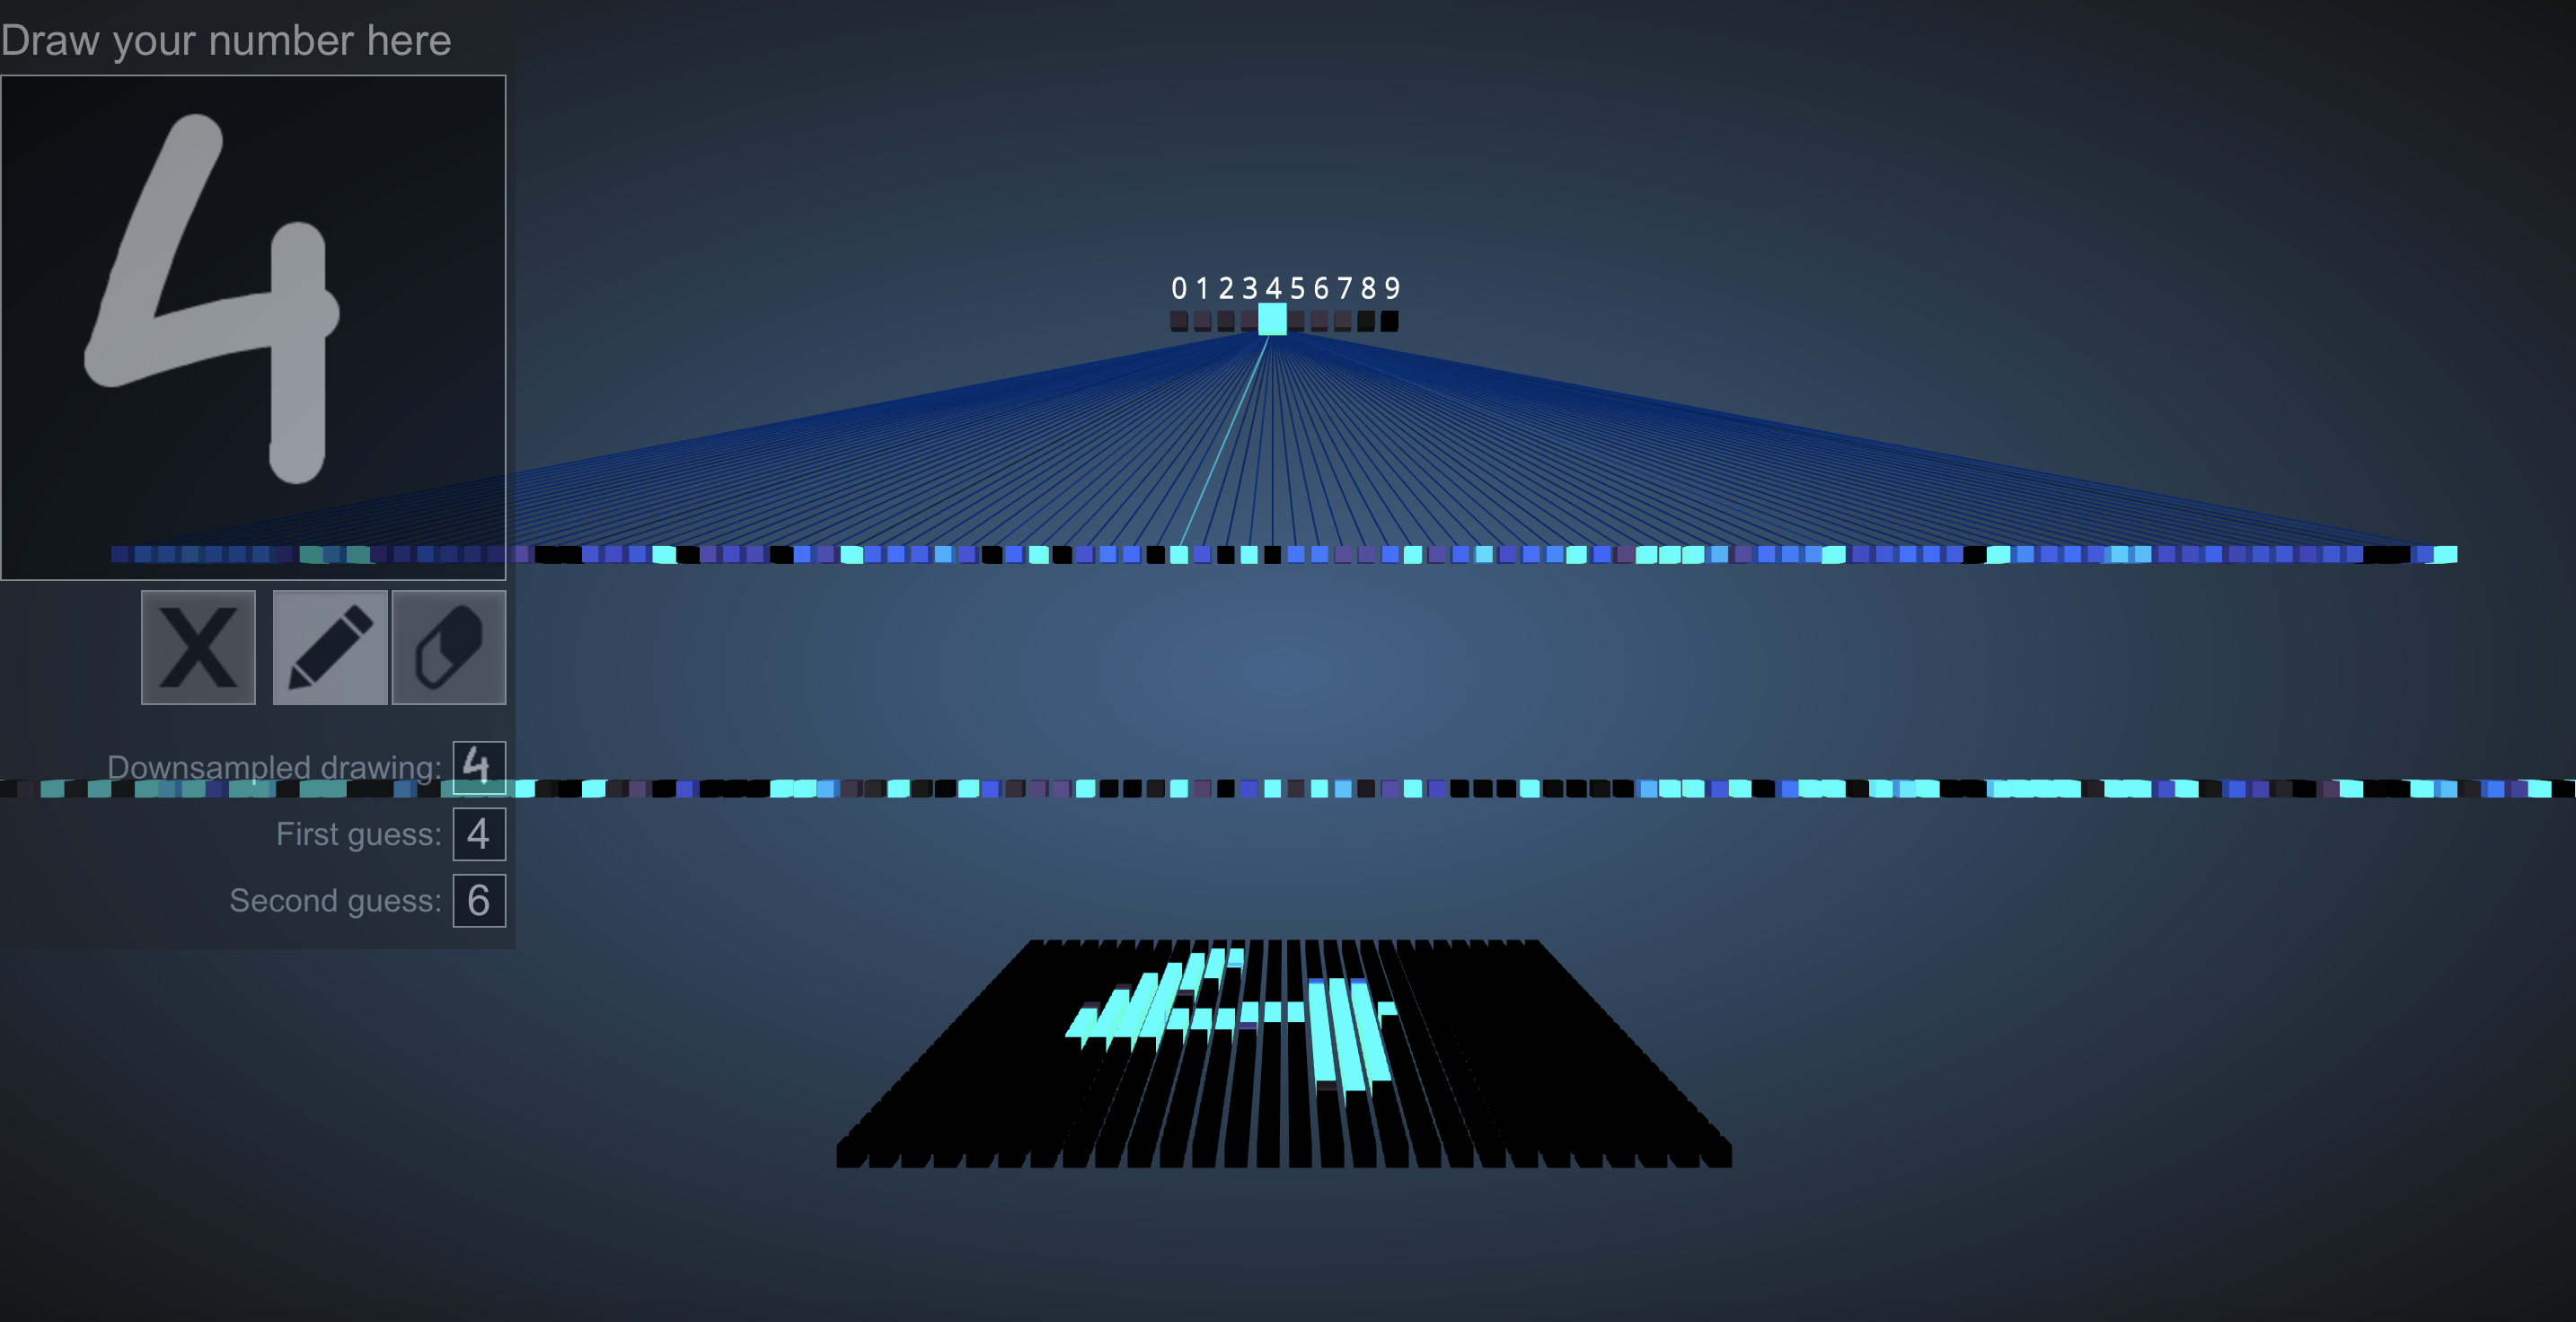
\includegraphics[width=12cm]{figures/Fully_Connected_MLP_3D.png}
\caption{2D Visualisation of a fully connected MLP \cite{harley2015isvc}}
\label{fig:cnn5}
\end{figure}

This MLP network has 784 nodes on the bottom layer (corresponding to pixels), 300 nodes in the first hidden layer, 100 nodes in the second hidden layer, and 10 nodes in the output layer (corresponding to the 10 digits)\cite{harley2015isvc}. \newline\newline
A brighter colour corresponds to a node which has a higher output value than others. In the input layer, the bright nodes are the ones receiving higher numerical pixel values as input. In the output layer, the only bright node corresponds to the digit 4, indicating that the MLP has correctly classified the input digit as 4.

\subsection{Convolutional Neural Networks}
\label{sect5_1_2}
CNNs are quite similar to regular neural networks – they are composed of neurons possessing learnable weights and biases; neurons get inputs, perform dot products and follow it up with non-linearity (optionally). The network expresses a single differentiable score function: from the raw image pixels on one end to class scores at the other. There is a loss function on the last, fully-connected which generates the final output. The difference exists for the type of input CNN architectures explicitly assume, which are images, allowing certain properties to be encoded into the architecture. These then make the forward function more efficient to implement and hugely decrease the number of parameters in the network \cite{cnn_stanford}.

\subsubsection{Architecture}
\label{sect5_1_2_1}
CNNs are biologically-inspired variants of MLPs. 



\subsubsection{Visualisation}
\label{sect5_1_2_2}
Along with visualising \ac{MLP}, Andy Harley developed a visualisation tool for a CNN trained to recognise the handwritten digits from the MNIST database \cite{harley2015isvc} as well. \newline\newline
This CNN has 1024 nodes on the bottom layer (corresponding to pixels), six 5x5 (stride 1) convolutional filters in the first hidden layer, followed by sixteen 5x5 (stride 1) convolutional filters in the second hidden layer, then three fully-connected layers, with 120 nodes in the first, 100 nodes in the second, and 10 nodes in the third. The convolutional layers are each followed by a downsampling layer that does 2x2 max pooling (with stride 2)\cite{harley2015isvc}. \newline\newline
The following figure shows how this network can be visualised in 2D.

\begin{figure}[h!]
\centering
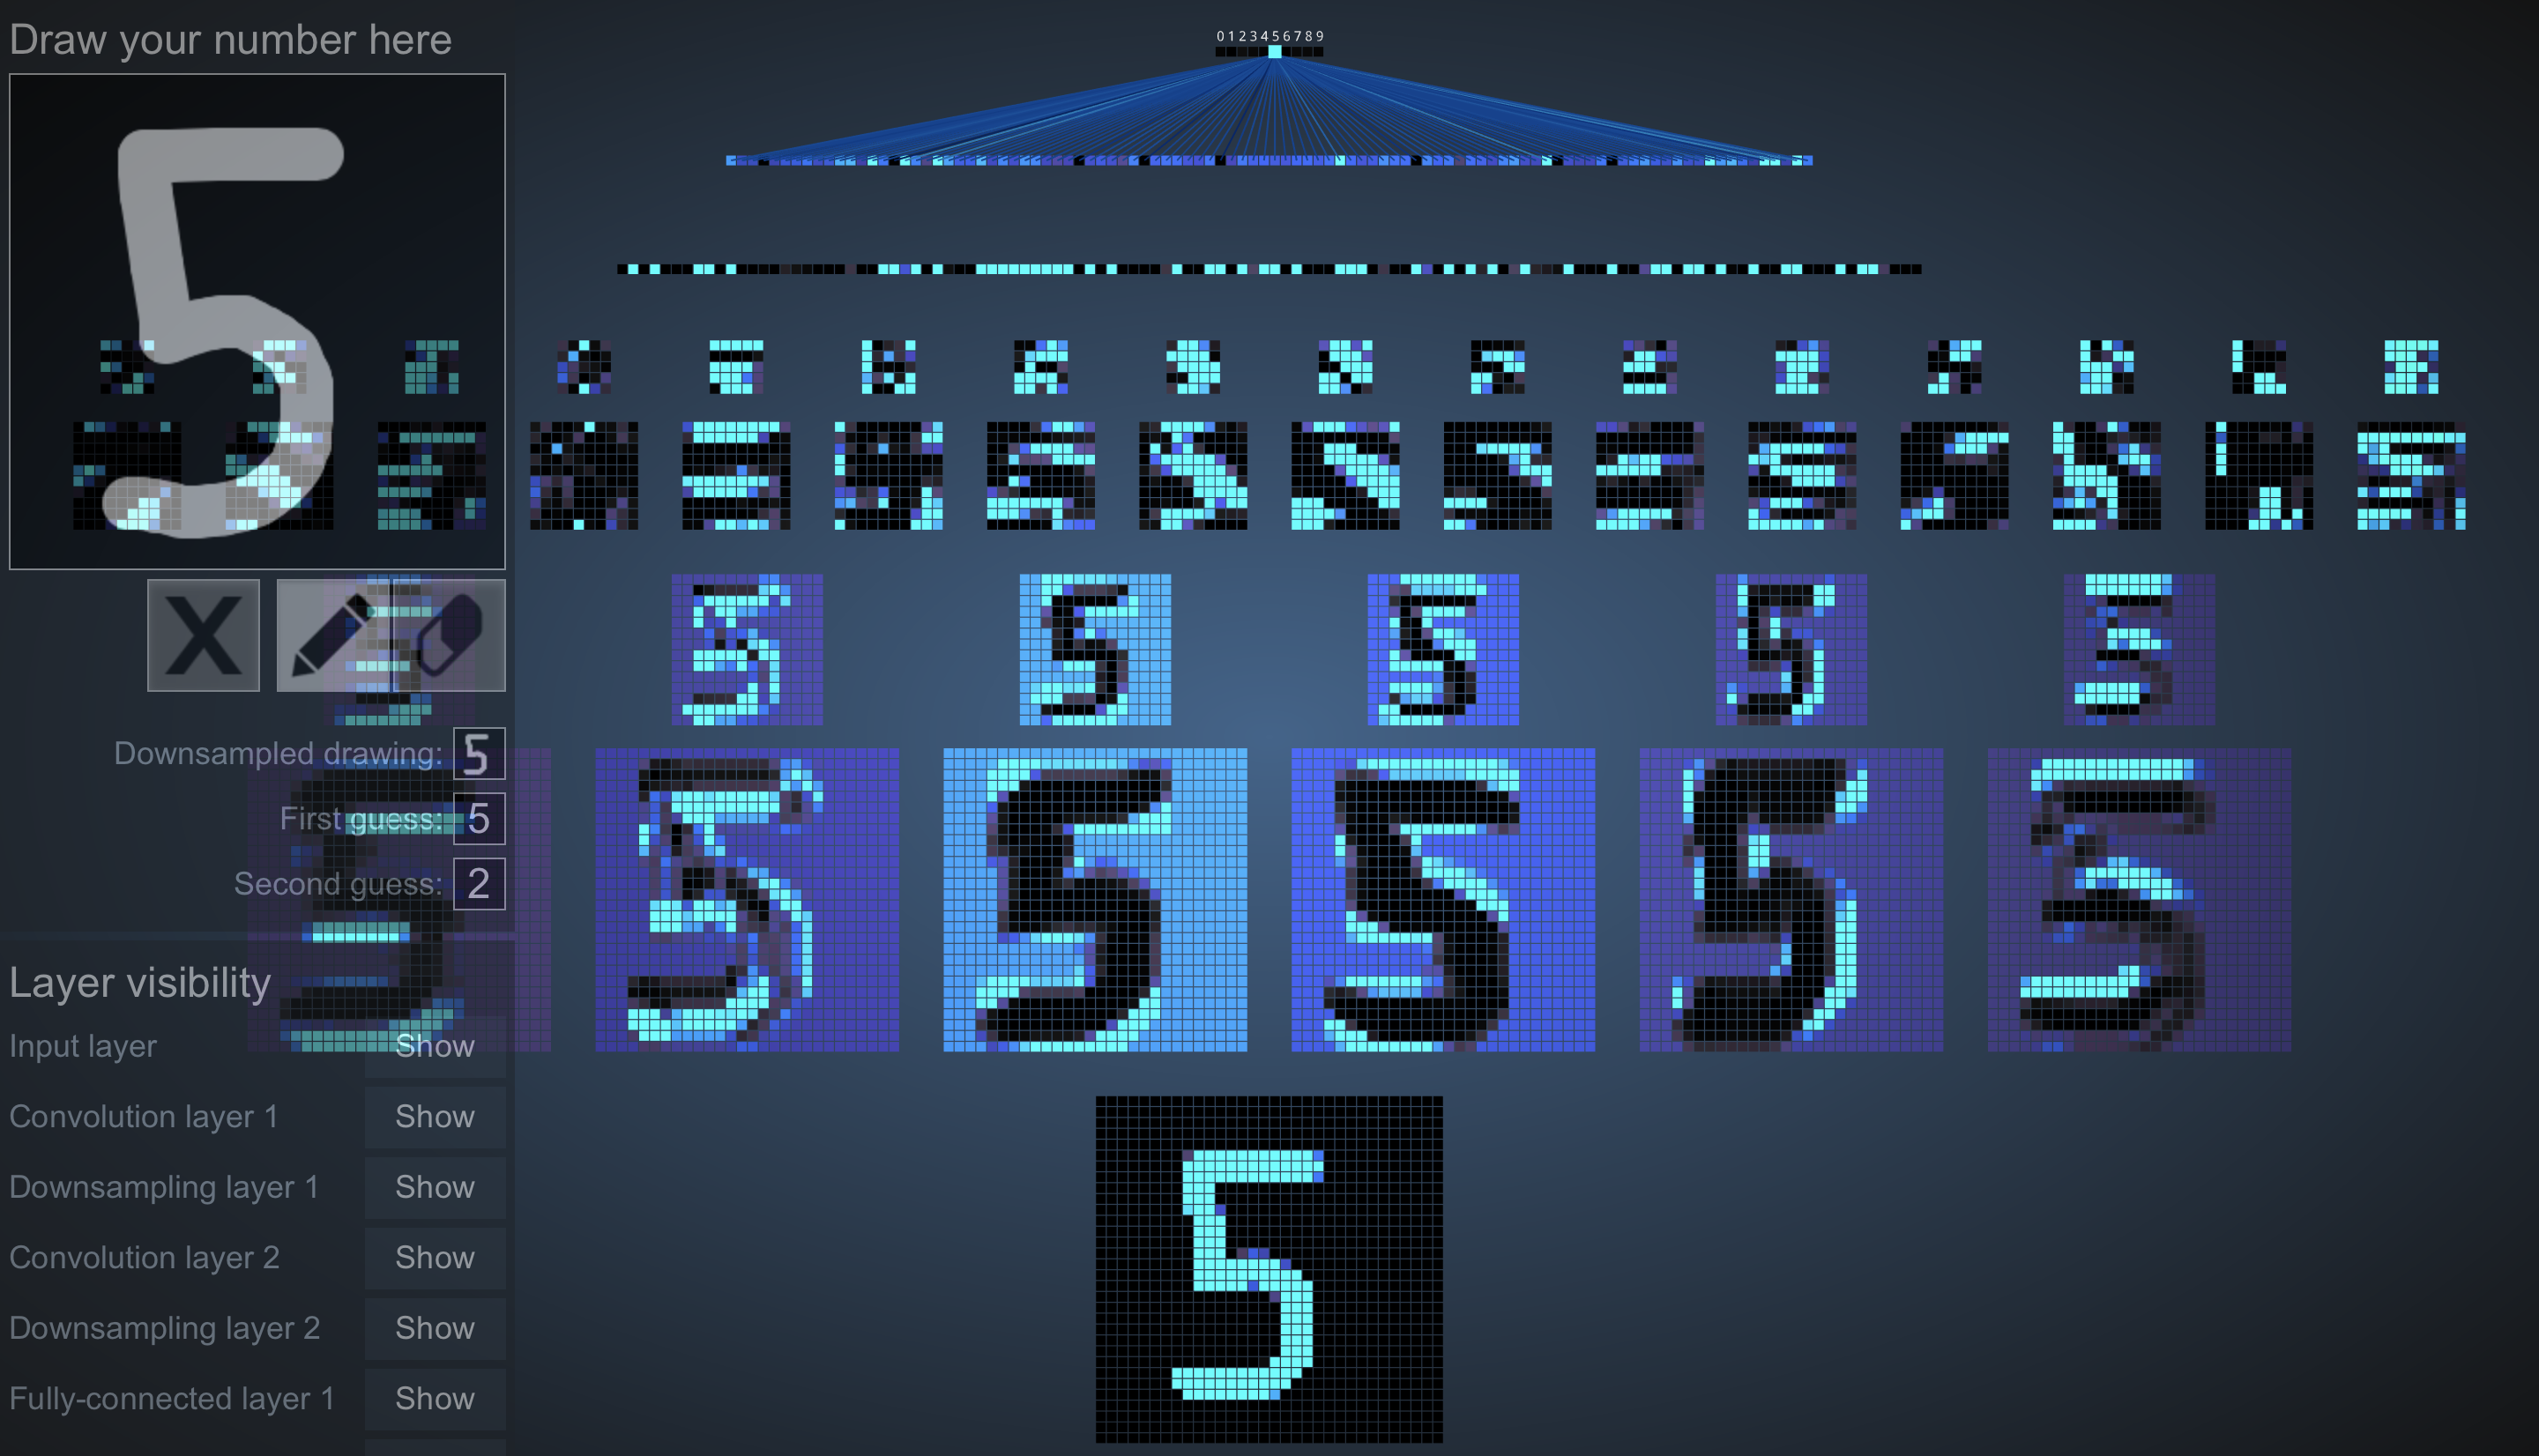
\includegraphics[width=13cm]{figures/ConvNet_2D.png}
\caption{2D Visualisation of a CNN recognising MNIST handwritten digits \cite{harley2015isvc}}
\label{fig:cnn6}
\end{figure}

\section{MNIST Database}
\label{sect5_2}
The \ac{MNIST} database is an enormous database of handwritten digits which is frequently utilized for training different image processing procedures \cite{mnist_wiki}. It is also extensively used for training and testing in the field of machine learning. \newline\newline 
The MNIST database consists of 60,000 training and testing images \cite{mnist_kus_ernst}. Samples from National Institute of Standards and Technology’s (NIST) original training and testing dataset were remixed to generate the MNIST database. The digits have been size-normalized and centered in a fixed-size image of 20x20 while preserving their aspect ratio \cite{cnn_lecun_mnist_app}. The resulting images contain grey levels because of anti-aliasing methods used by the normalization algorithm. The images were centred in a 28x28 image by calculating the centre of mass of the pixels and rendering the image to place this point at the centre of the 28x28 field. \newline\newline
The database is a good starting point for individuals who desire to learn machine learning techniques and pattern recognition methods on real-world data while spending marginal efforts on preprocessing and formatting. When one learns how to program, there's a tradition to print "Hello World" in his first program. Similar to how programming has Hello World, machine learning has MNIST. \newline\newline
A number of scientific papers have been written to attempt achieving the lowest error rate in predicting the digits – one paper achieves a rate as low as 0.23 percent using a hierarchical system of convolutional neural networks.

\section{Experiments}
\label{sect5_3}
An existing real word application was obtained and executed to further gauge the performance capabilities of OpenCL. An MNIST handwritten digits prediction application written by Gopala Krishna Hegde based on LeNet-5 convolutional neural networks was cloned from GitHub for this purpose \cite{cnn_mnist_papaa}. The implementation has been done in C++ as well as OpenCL.

\subsection{Results}
\label{sect5_3_1}
The MNIST handwritten digit recognition application was executed on different devices - three CPUs and two GPUs, and average timings were calculated for different parts in the execution of kernels. There is a total of eight kernels executing on the device, launched by the host one after the other. The kernels launched have a work dimension of 3 and their global sizes are (12, 12, 20). \newline\newline
The following results were obtained on Intel(R) Core(TM) i5-5200U CPU, Intel(R) Xeon(R) E5-1650 CPU, and NVIDIA Quadro 600 GPU.

\begin{table}[h!]
\centering
 \caption{Execution time (in µs) for different operations in MNIST Application on different devices}
 \vspace{3mm}
 \renewcommand\arraystretch{1.6}
 \begin{tabular}{ | m{7em} | r | r | r | r | r |  }
 \hline
 \multicolumn{6}{|c|}{MNIST Application OpenCL Execution Times} \\
 \hline
 \multicolumn{1}{|c|}{\bfseries Device} & \multicolumn{1}{c|}{\bfseries i3-2350M} & \multicolumn{1}{c|}{\bfseries i5-5200U} & \multicolumn{1}{c|}{\bfseries E5-1650} & \multicolumn{1}{c|}{\bfseries Quadro 315M} & \multicolumn{1}{c|}{\bfseries Quadro 600} \\
 \hline
 Initialize Application & & 0.9 & 1.3 & & 1.5 \\
 \hline
 Allocate Host Memory & & 16.2 & 16.9 & & 16.5 \\
 \hline
 Initialize Device & & 62198.5 & 78408.9 & & 36985.2 \\ 
 \hline
 Build Kernel & & 132807.2 & 130634.2 & & 16914.6 \\
 \hline
 Allocate Device Memory & & 833.2 & 1025.2 & & 1364.7 \\
 \hline
 Kernel Execution &1223.8 & 299.3 &  397.7 & 15581.6 & 3903.5 \\
 \hline
 \end{tabular}
 \label{table:mnist_gpu}
\end{table}
%Kernel Execution &12223.8 & 16251.4 & 18930.7 & 15581.6 & 3903.5 \\
Also, the sequential code written in C++ was executed on two CPUs and average execution times were measured. The following results were obtained on Intel(R) Core(TM) i3-2350M and Intel(R) Xeon(R) E5-1650 CPUs. 

\begin{table}[h!]
\centering
 \caption{Execution time (in µs) for sequential execution of MNIST Application on different CPUs}
 \vspace{3mm}
 \renewcommand\arraystretch{1.5}
 \begin{tabular}{ | l | r | r | }
 \hline
 \multicolumn{1}{|c|}{\bfseries Device} & \multicolumn{1}{c|}{\bfseries i3-2350M} & \multicolumn{1}{c|}{\bfseries E5-1650} \\
 \hline
 Execution Time & 85523 & 33892 \\
 \hline
 \end{tabular}
 \label{table:mnist_cpu}
\end{table}

\subsection{Discussion}
\label{sect5_3_2}
The results above in Table \ref{table:mnist_gpu} show the time taken on three different processors for initializing the application, allocating memory in the host, initializing the device on which the kernels will execute on, building the kernels, allocating memory on the device, and the execution of all kernels. The numbers in Table \ref{table:mnist_cpu} indicate the time taken by the CPU to compute the digit recognition results sequentially.  \newline\newline
Comparing the timing values for the CPUs from Tables \ref{table:mnist_cpu} and \ref{table:mnist_gpu}, the extent of parallelism introduced by OpenCL can be evidently noticed. There is a speedup of 69 times for Intel(R) Core(TM) i3-2350M and 85 times for Intel(R) Xeon(R) E5-1650. 
\newline\newline
%From the results, it is evident that both the CPUs, i5-5200 and Xeon E5-1650 take much lesser time than the NVIDIA Quadro 600 GPU in the kernel execution – their performance is 10.6 and 9.89 times better than the GPU’s. This could be reasoned by making the point that OpenCL parallelizes the code on both the CPUs and GPU, but the execution is not parallel enough to exploit the full usage of the GPU’s performance capabilities. Also, the kernel execution time is for the completion of all the kernels, between which data transfers take up more time as compared to the CPU. The host and the target being CPU and GPU, respectively, increase the communication bottleneck drastically and leads directly to having a greater execution time for the GPU. In case of the CPUs, the communication requires hardly any time, leading to a smaller execution time. \newline\newline